\emph{EiffelStudio}, as well as \emph{EiffelMedia}, come with an installer. Just follow the onscreen instructions like you would when installing any other program. No magic there..\\

\emph{TRAFFIC} does not need to be installed, just download the zip-file and unzip it to a directory of your choice.\\ 
Flat Hunt is located in the directory \texttt{traffic/example/flat\_hunt}. To get it to run, however, you'll have to compile it first.\\

For that you have to complete the following steps:

\begin {enumerate}
	\item{Start EiffelStudio}
	\item{Click on "File ->New Project...". Choose "Open existing Ace (control file)" from the dialog (see \autoref{newproject}) and click on "Next".
\begin{figure}[h]
\centerline{\hbox{  
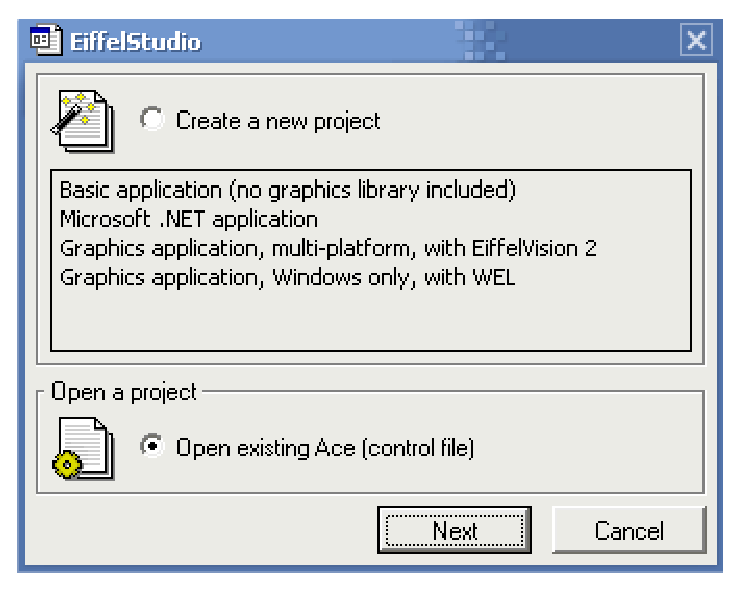
\includegraphics[width=80mm]{new_project}
  }}
\caption{New Project Dialog}
\label{newproject}
\end{figure}	  
}
	\item {This will open a file dialog that lets you choose the Ace file. Browse to the directory \texttt{traffic/example/flat\_hunt}. Depending on the operating system you are working on, choose \emph{ise\_windows.ace} or \emph{ise\_linux.ace}. Click on "Open". }
	\item{The dialog shown in \autoref{choosedir} lets you choose the project directory. In most cases you can leave both paths (Ace file and location) as EiffelStudio proposes. Make sure that the checkbox for compiling the generated project is selected. Click on "OK". This will start the compilation of the project.
\begin{figure}[h]
\centerline{\hbox{  
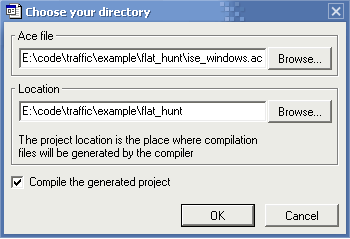
\includegraphics[width=80mm]{choose_directory}
  }}
\caption{Project Directory Dialog}
\label{choosedir}
\end{figure}
}
	\item{Once the project is compiled you can execute it by clicking on the "Launch" button in EiffelStudio or by hitting \textbf{F5}.}
\end {enumerate}

Now you are ready for playing Flat Hunt. Enjoy\ldots 

